% Copyright (c) 2023-2026 Oriol Cayon, Delft University of Technology
% SPDX-License-Identifier: Apache-2.0
\documentclass[11pt,a4paper]{article}

\usepackage[margin=2.4cm]{geometry}
\usepackage{graphicx}
\usepackage{amsmath,amssymb}
\usepackage{booktabs}
\usepackage{xcolor}
\usepackage{caption}
\usepackage{float}
\usepackage{enumitem}
\usepackage{fancyhdr}
\usepackage[hidelinks]{hyperref}
\usepackage{siunitx}

\graphicspath{{figures/}}
\captionsetup{font=small,labelfont=bf}
\setlist{itemsep=2pt,parsep=0pt,topsep=3pt}

\pagestyle{fancy}
\fancyhf{}
\fancyhead[L]{\small\textsc{AWETrim --- winch model}}
\fancyhead[R]{\small\thepage}
\renewcommand{\headrulewidth}{0.3pt}

\newcommand{\code}[1]{\texttt{\small #1}}

\title{\vspace{-1.5cm}\textbf{The winch model in AWETrim}\\[4pt]
  \large Force law, drum inertia and drivetrain friction}
\date{}

\begin{document}
\maketitle
\vspace{-1.2cm}

\section{Model}

The kite is quasi-steady: at each instant its force balance gives the tether
tension $T$ at the ground for a given reel speed $v_r$. The winch closes the
radial direction. Between the tether and the motor sits the drivetrain: drum,
gearbox and motor, all referred to the tether. The drum obeys
\begin{equation}
  m\,\dot v_r = T - F_f(v_r, T) - F_m ,
  \label{eq:drum}
\end{equation}
with $F_m$ the motor (generator) force, $m$ the rotating inertia seen at the
tether and $F_f$ the friction:
\begin{align}
  m &= J \left(\frac{n}{r_d}\right)^{2}, &
  F_f &= (F_c + k\,T)\tanh\!\left(\frac{v_r}{\varepsilon}\right) + c_v\, v_r .
  \label{eq:params}
\end{align}
$J$ is the total inertia on the motor side, $n$ the gear ratio and $r_d$ the
drum radius. $F_c$ is the Coulomb friction, $c_v$ the viscous coefficient and
$k$ an optional load-proportional part (pulleys, belt, gear mesh). The $\tanh$,
with $\varepsilon = \SI{0.05}{m.s^{-1}}$, smooths the sign of $v_r$, so the
model stays twice differentiable where $v_r$ changes sign.

\paragraph{The force law sets the motor force.} The winch controller is a
torque-controlled machine: its law $F_\mathrm{law}(v_r, u_p)$ (linear or
quadratic in $v_r$, soft-capped at the force limits, offset by the depower
$u_p$) is the force the motor applies. With Eq.~\eqref{eq:drum}, the tension
the kite feels is
\begin{equation}
  T = F_\mathrm{law}(v_r) + F_f(v_r) + m\,\dot v_r .
  \label{eq:law}
\end{equation}
Friction raises the tension during reel-out and lowers it during reel-in;
inertia adds tension while the drum accelerates. With $m = F_c = c_v = k = 0$
(the default) Eq.~\eqref{eq:law} is the ideal winch, $T = F_\mathrm{law}$.

\paragraph{Shaft power.} The power at the motor is
\begin{equation}
  P_m = F_m v_r = T v_r - \underbrace{v_r F_f}_{\ge 0}
        - \frac{\mathrm{d}}{\mathrm{d}t}\!\left(\tfrac12 m v_r^2\right).
\end{equation}
Friction is lost in both reel directions. The inertia term is the drum's
kinetic energy: it is returned over a closed cycle, so on a periodic cycle
inertia changes the mean power only through the force limits.

\section{Discretisation}

\paragraph{Forward simulation.} The march solves, at each node, the kite's
force balance and Eq.~\eqref{eq:law} for $(T, u_s, \dot s, v_r)$. The drum's
time constant, $m$ over the slope of the law (\SI{\sim 0.06}{s} for the LEI-V3),
is far shorter than a node step (\SI{\sim 0.3}{s}), so $\dot v_r$ is the
backward difference to the previous node (implicit Euler),
$\dot v_r \approx (v_{r,i} - v_{r,i-1})/\Delta t_{i-1}$. The previous reel speed
and $1/\Delta t$ enter the node solver as two parameters; the first node starts
with a steady drum.

\paragraph{Optimisation.} The cycle NLP uses the same model. Its objective is
the mean shaft power, with the inertia part written as the exact change of
$\tfrac12 m v_r^2$ over each interval, so it telescopes. With the force law
(\code{winch\_mode: force\_law}) Eq.~\eqref{eq:law} replaces the law row, with
the same backward difference as the march. With a free reel speed
(\code{free\_speed}) the motor force
$F_m = T - F_f - m\dot v_r$ is held below \code{max\_tether\_force}.

\section{Parameters and use}

\begin{table}[H]
\centering\small
\caption{LEI-V3 drivetrain: the TU Delft GS1 drivetrain as V3Kite.jl flies it
(\code{sim\_settings\_reelout.yaml}, the KiteUtils defaults; Fechner 2016,
Table 4.1). Stored tether-referred in \code{system.yaml}, \code{drums[0]}.}
\begin{tabular}{lll}
\toprule
Quantity & \code{system.yaml} key & Value \\
\midrule
Inertia at the tether, $0.204\,(6.2/0.1615)^2$ & \code{inertia\_equivalent\_mass} & \SI{300.7}{kg} \\
Coulomb friction $F_c$ & \code{friction\_coulomb} & \SI{122}{N} \\
Viscous friction $c_v$ & \code{friction\_viscous} & \SI{30.6}{N.s.m^{-1}} \\
Load fraction $k$ (not in V3Kite) & \code{friction\_load\_fraction} & 0.0535 \\
\bottomrule
\end{tabular}
\end{table}

\noindent The drivetrain is off unless \code{sim\_parameters} asks for it:
\code{winch\_drivetrain: true} takes $m$, $F_c$ and $c_v$ from the system file;
\code{winch\_inertia\_mass}, \code{winch\_friction} and
\code{drivetrain\_load\_fraction} set the parts one by one (\code{true} or a
value). The cycle script takes \code{--winch-drivetrain}. Code:
\code{awetrim.system.winch.Drivetrain} and \code{Winch.radial\_equation}.

\section{Example}

Figure~\ref{fig:sim} marches the \SI{9}{m.s^{-1}} LEI-V3 cycle with its force
law, without optimising. The motor force stays at the law's limit while the
tension reaches \SI{8.87}{kN}, the extra being friction (\SI{\sim 0.23}{kN} in
reel-out) and the drum accelerating into reel-out (up to \SI{0.74}{kN}). The
mean shaft power is \SI{9.8}{kW}, against \SI{11.0}{kW} at the tether.

\begin{figure}[H]
  \centering
  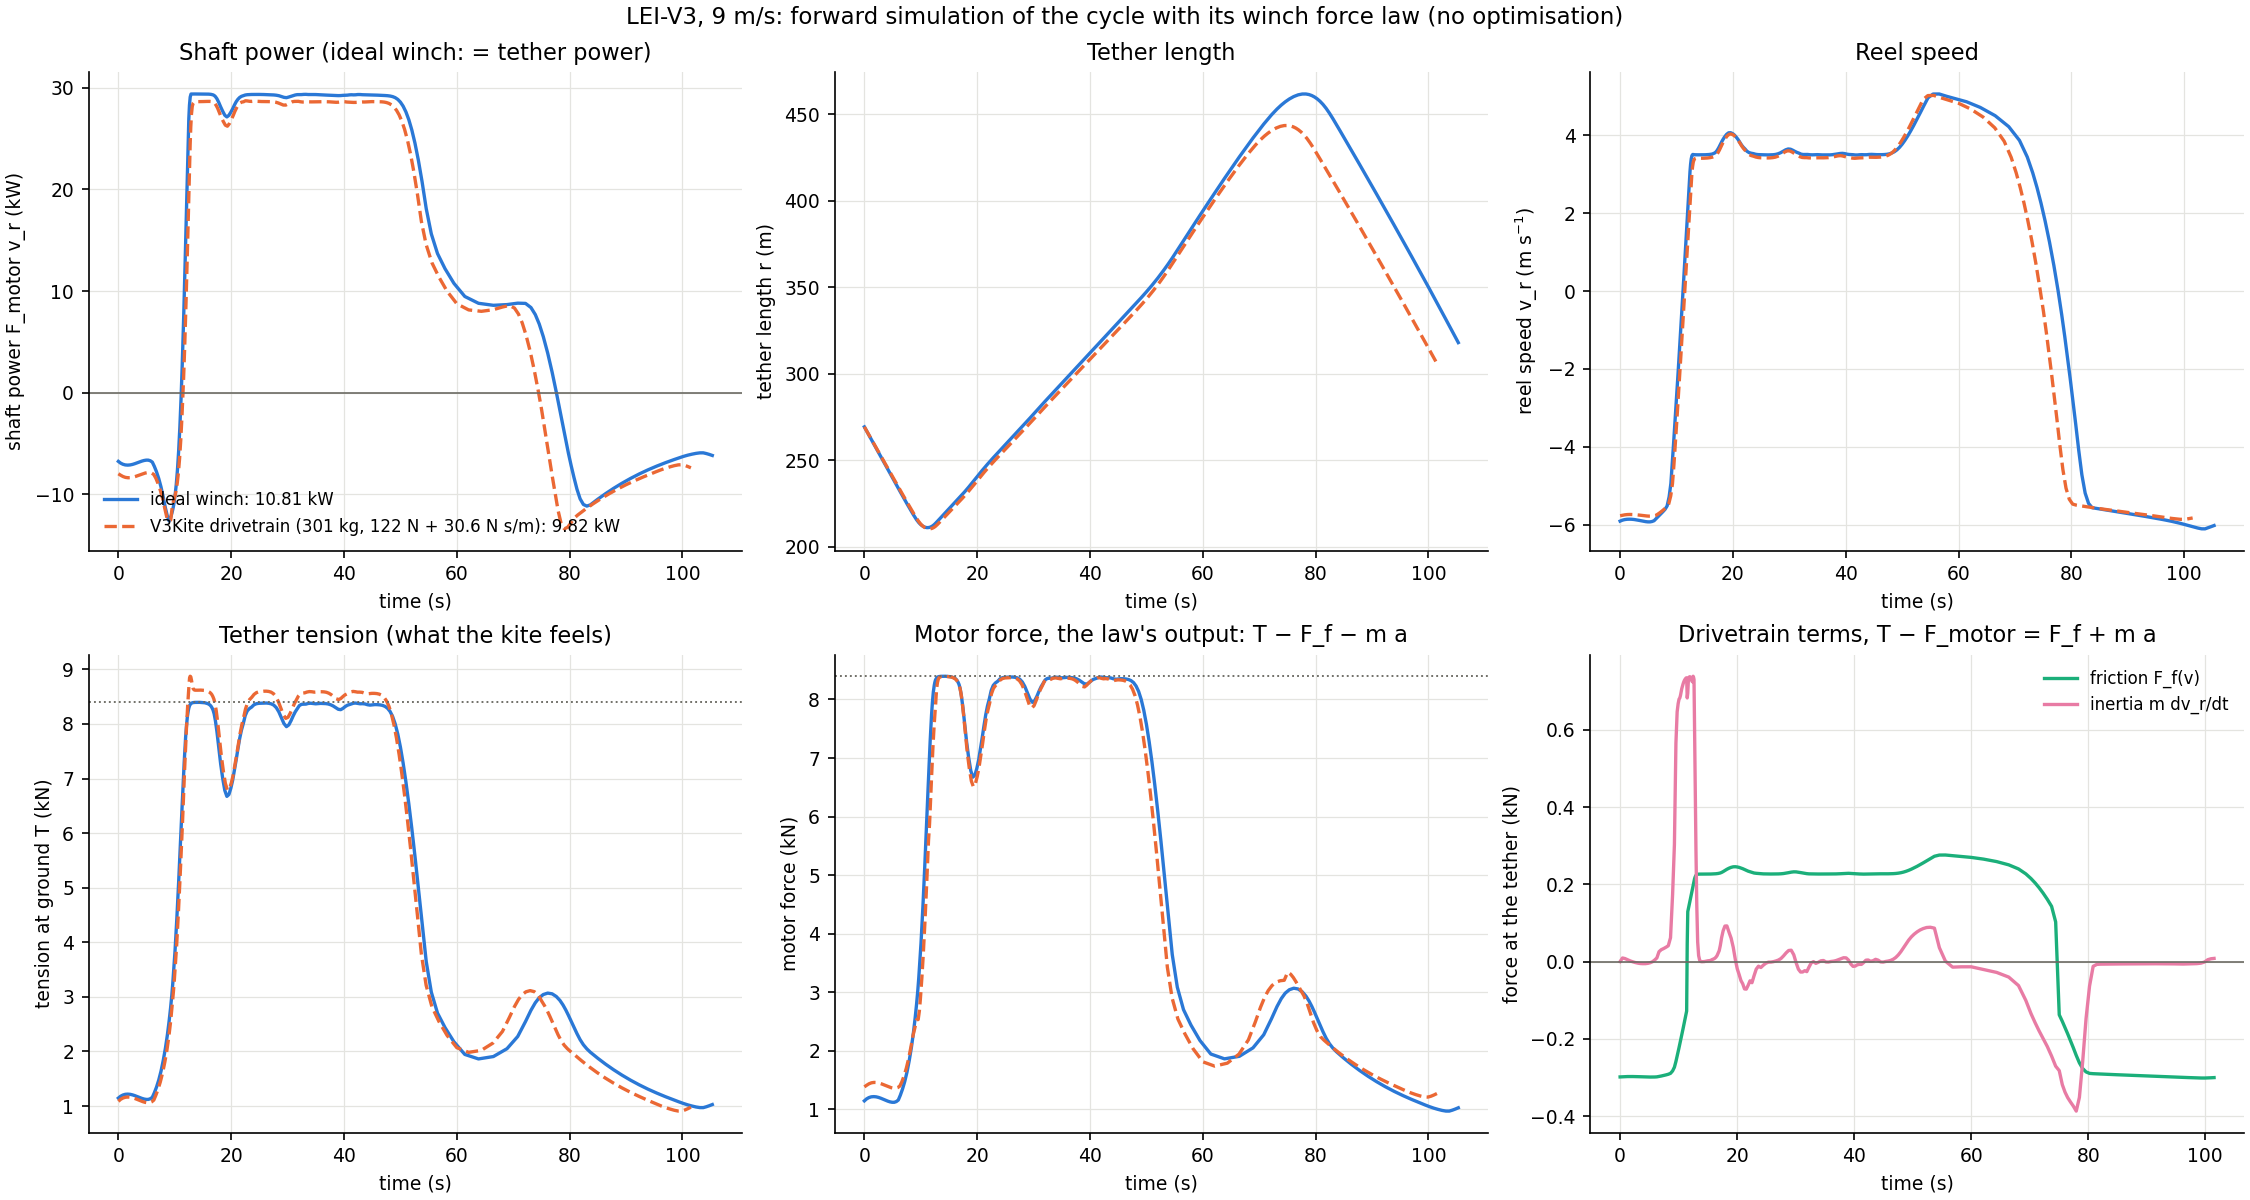
\includegraphics[width=\linewidth]{winch_drivetrain_sim.png}
  \caption{Forward simulation of the \SI{9}{m.s^{-1}} cycle path with an ideal
  winch and with the LEI-V3 drivetrain (Table~1).}
  \label{fig:sim}
\end{figure}

\end{document}
